\section{The Data}\label{sec:data}



\subsection{Universal Corpus and Data Structure} \label{sec:structure}

Building on their previous paper, \newcite{abney2011data} describe the data structure they envisage for the universal corpus in more detail, and we aim to adopt this structure where possible.  Two types of text are distinguished:

\textbf{Aligned texts} consist of multiple parallel documents, aligned at the document, sentence, or word level. The collection of parallel documents as a whole is assigned a unique identifier, with each individual document labelled by this identifier and the corresponding language code.  A monolingual document is simply one with only a single associated language code.  Sentences and words within documents are also assigned identifiers (relative to the document), if alignment has been performed at that level.

\textbf{Analysed texts}, in addition to the raw text, contain more detailed annotations including parts of speech, morphological information, and syntactic relations.  This is stored as a table, where rows represent words, and columns represent the following types of information: document ID, language code, sentence ID, word ID, wordform, lemma, morphological information, part of speech, gloss, head/governor, and relation/role.

Out of our data sources, three can be straightforwardly represented in their aligned text structure. However, ODIN contains richer annotations, which are in fact difficult to fit into their proposal, and which we discuss in section \ref{sec:odin} below.


\subsection{Data Sources} \label{sec:sources}

Although data size matters in general NLP, \emph{universality} is the top priority for a universal corpus. We focus on the following data sources, because they include a large number of languages, include several parallel texts, and demonstrate a variety of data types which a linguist might encounter (structured, semi-structured, unstructured): Online Database of Interlinear Text (ODIN), Omniglot website, Universal Declaration of Human Rights (UHDR), and Wikipedia.

Our resulting corpus runs the full gamut of text types outlined by Abney and Bird, ranging from single-language text (Wikipedia) to parallel text (UDHR and Omniglot) to IGTs (ODIN). Table~\ref{table:corpus} gives some coverage statistics, and we describe each source in the following subsections.  For 332 languages, the corpus contains data from more than one source.


\begin{table}[t]
\small
\centering
    \begin{tabular}{l|rr|rr}
    ~         				& Langs. 	& Families 	& Tokens		& Size	\\ \hline
    ODIN      				& 1,270      & 100       		& 351,161		& 39 MB		\\
    Omniglot  				& 129        & 20        		& 31,318		& 677 KB	\\
    UDHR      				& 352        & 46        		& 640,588		& 5.2 MB	\\
    Wikipedia 				& 271        & 21       		&				& 37 GB\\ \hline
    \textbf{Combined}	    & 1,451	    & 105 
    \end{tabular}
\caption{Corpus Coverage}
\label{table:corpus}
\end{table}



\paragraph{Universal Declaration of Human Rights.}

The Universal Declaration of Human Rights (UDHR) is a document released by the United Nations in 1948, and represents the first global expression of human rights. It consists of 30 articles, amounting to about four pages of text. This is a useful document for NLP, since it has been translated into a wide variety of languages, providing a highly parallel text.


\paragraph{Wikipedia.}

Wikipedia is a collaboratively-edited encyclopedia, appealing to use for NLP because of its large size and easy availability. At the time of writing, it contained 30.8 million articles in 286 languages, which provides a sizeable amount of monolingual text in a fairly wide range of languages. Text dumps are made regularly available, and can be downloaded from \url{http://dumps.wikimedia.org}.

\paragraph{Omniglot.}

The Omniglot website\footnote{\url{http://www.omniglot.com}} is an online encyclopedia of writing systems and languages. We extract information from pages on \emph{`Useful foreign phrases'} and the \emph{`Tower of Babel'} story, both of which give us parallel data in a reasonably large number of languages. % The urls for these resources are:

\paragraph{ODIN.} \label{sec:odin}

ODIN (The Online Database of Interlinear Text) is a repository of
interlinear glossed texts (IGTs) extracted from scholarly documents
\cite{lewis2006odin,lewis2010odin}.  Compared to other resources, it
is notable for the breadth of languages included and the level of
linguistic annotation.  An IGT canonically consists of three lines:
(i) the source, a sentence in a target language, (ii) the gloss, an
analysis of each source element, and (iii) the translation,
done at the sentence level. The gloss line can additionally include a
number of linguistic terms, which means that the gloss 
%can more
%properly described as being written in a metalanguage, rather than a
is written in metalanguage rather than natural language.  In ODIN, translations are into English, and glosses
are written in an English-based metalanguage.  An accepted set of
guidelines are given by the Leipzig Glossing
Rules,\footnote{\url{http://www.eva.mpg.de/lingua/resources/glossing-rules.php}}
where morphemes within words are separated by hyphens (or equal signs,
for clitics), and the same number of hyphens should appear in each
word of the source and gloss.

The data from ODIN poses the first obstacle to straightforwardly adopting Abney and Bird's data structure. 
The proposed data structure for the universal corpus is aligned at the word level, and includes a specific list of relevant features which should be used to annotate words. When we try to adapt IGTs into this format, we run into certain problems.  Firstly, there is the problem that the most fundamental unit of analysis according to the Leipzig Glossing Rules is the morpheme, not the word.  Ideally, we should encode this information explicitly in a universal corpus, assigning a unique identifier to each morpheme (instead of, or in addition to each word). Indeed, \newcite{haspelmath2011segment} argues that there is no cross-linguistically valid definition of \textit{word}, which undermines the central position of words in the proposed data structure.

Secondly, it is unclear how to represent the gloss.  Since the gloss line is not written in a natural language, we cannot treat it as a simple translation.  However, it is not straightforward to incorporate it into the proposed structure for analysed texts, either.  
% We could simply always map the gloss to the \textsc{gloss} field, but this would run against the suggestion that this field should "contain symbols from controlled vocabularies".  Indeed, this information might be more suited to the \textsc{morph, pos,} or \textsc{rel} fields, but it would be difficult to automatically process ODIN to determine which morphemes should be assigned to which field.
One possible resolution is to move all elements of the gloss written in capital letters to the \textsc{morph} field (as functional elements are usually annotated in this way), and all remaining elements to the \textsc{gloss} field.  However, this loses information, since we no longer know which morpheme has which meaning.  To keep all information encoded in the IGT, we need to modify \newcite{abney2011data}'s proposal.

The simplest solution we can see is to allow morphemes to be a level of structure in the universal corpus, just as documents, sentences, and words already are.  The overall architecture remains unchanged.  We must then decide how to represent the glosses.

Even though glosses in ODIN are based on English, having been extracted from English-language documents, this is not true of IGTs in general.  For example, it is common for documentary linguists working on indigenous languages of the Americas to provide glosses and translations based on Spanish.  For this reason, we believe it would be wise to specify the language used to produce the gloss.  Since it is not quite the language itself, but a metalanguage, one solution
would be to use new language codes that make it clear both that a metalanguage is being used, and also what natural language it is based on.  The five-letter code \texttt{gloss} cannot be confused with any code in any version of ISO 639 (with codes of length two to four).  Following the convention that subvarieties of a language are indicated with suffixes, we can append the code of the natural language.  For example, glosses into English and Spanish-based metalanguages would be given the codes \texttt{gloss-eng} and \texttt{gloss-spa}, respectively.

One benefit of this approach is that glossed texts are treated in exactly the same way as parallel texts.  There is a unique identifier for each morpheme, and glosses are stored under this identifier and the corresponding gloss code.  Furthermore, to motivate the important place of parallel texts in a universal corpus, Abney and Bird view translations into a high-resource reference language as a convenient surrogate of meaning. By the same reasoning, we can use glosses to provide a more detailed surrogate of meaning, only written in a metalanguage instead of a natural one.



\subsection{Representation and Universality} \label{sec:stats}

According to Ethnologue, there are 7105 living languages, and 147 living language families. Across all our data sources, we manage to cover 1347 languages in 106 families, which represents 19.0\% of the world's languages. To get a better idea of the kinds of languages represented, we give a breakdown according to their EGIDS scores (Expanded Graded Intergenerational Disruption Scale) \cite{lewis2010assessing} in Figure \ref{fig:heatmap}. The values in each cell have been colored according to proportion of languages represented, with green indicating good coverage and red poor. It's interesting to note that vigorous languages (6a) are poorly represented across all data sources, and worse than more endangered categories. In terms of language documentation, vigorous languages are less urgent goals than those in categories 6b and up, but this highlights an unexpected gap in linguistic resources.

\begin{figure*}[t]
\begin{centering}
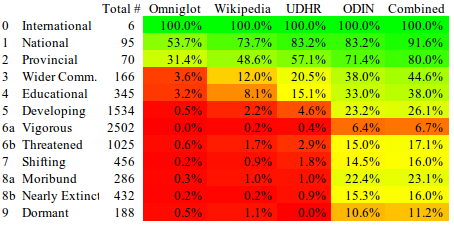
\includegraphics[scale=0.5]{heatmap2.png}
%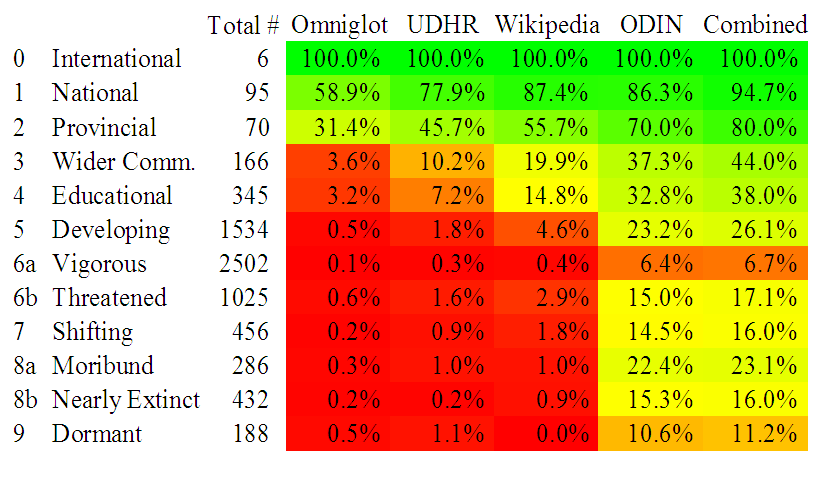
\includegraphics{heatmap-numbers.png}
\caption{Heatmap of languages in SeedLing according to endangerment status}\label{fig:heatmap}
\end{centering}
\end{figure*}
